\documentclass[12pt,a4paper]{article}
\usepackage[T2A]{fontenc}
\usepackage[utf8]{inputenc}
\usepackage[english,russian]{babel}
\usepackage{geometry,graphicx,amsmath,booktabs,float}
\geometry{margin=2cm}
\title{Фазовые портреты относительного движения по модели ХКУ}
\author{Задание 2}
\date{}
\begin{document}
\maketitle
\section{Связь с первым заданием и начальные условия}
В первом задании сравнивались модель Хилла--Клохесси--Уилтшира (ХКУ) и независимое двухтельное движение аппаратов. Для настоящей работы взяты три характерных набора из его таблицы: №1 ($x_0=0.1$ км, $v_{x0}=0$, $v_{y0}=-2nx_0$), №3 ($x_0=0.1$ км, $v_{x0}=0$, $v_{y0}=0.1$ км/с) и №65 ($x_0=100$ км, $v_{x0}=v_{y0}=0.1$ км/с). Во всех трёх $y_0=0$. Номер обозначает базовый случай первого задания; здесь к нему добавляется поперечное движение, поэтому итоговые начальные условия отличаются от строк первого задания.

Опорная орбита круговая, $a=7000$ км, $\mu=398600.4418$ км$^3$/с$^2$, $i=51.6^\circ$, $\Omega=30^\circ$, $n=\sqrt{\mu/a^3}$. Для каждого базового случая построена сетка: разность наклонений $\Delta i=0.01^\circ,0.1^\circ,0.5^\circ$ и истинная аномалия $\nu_0=0^\circ,90^\circ,180^\circ,270^\circ$. Итого 36 вариантов. Два состояния сначала получены в инерциальной системе из элементов круговых орбит; разность проецируется в систему RTN с учётом вращения скорости. Затем компоненты $z_0,\dot z_0$, порождённые разностью наклонений, сохраняются, а $x_0,y_0,\dot x_0,\dot y_0$ заменяются значениями базового случая. Полученное состояние переводится обратно в инерциальную систему для сравнения с двухтельным расчётом.

\section{Метод сравнения}
Расчёт проводится на интервале двух периодов опорной орбиты с 721 точкой, включая границы, как в первом задании. В ХКУ используются уравнения
\[\ddot x-2n\dot y-3n^2x=0,\quad \ddot y+2n\dot x=0,\quad \ddot z+n^2z=0.\]
Они решаются аналитически. Для сравнения два аппарата независимо интегрируются по уравнениям центрального поля $\ddot{\mathbf r}=-\mu\mathbf r/|\mathbf r|^3$ с относительным и абсолютным допуском $10^{-10}$. Разность их положений переводится в RTN. Ошибка — норма разности положений двух моделей в одинаковые моменты. Для ориентировочной оценки применимости приводится максимум двухтельного расстояния $\rho$ относительно $a$; это не установленная граница допустимой ошибки.

\section{Результаты}
В таблице указаны диапазоны максимальной ошибки по четырём аномалиям и наибольшее $\rho/a$ на интервале для каждой комбинации базового случая и наклонения.
\begin{center}\small
\begin{tabular}{rrrr}\toprule
Случай & $\Delta i$, град & Ошибка, км & $\max\rho/a$ \\\midrule
1 & 0.01 & 0.0040--0.0043 & 0.00018 \\
1 & 0.1 & 0.4018--0.4022 & 0.00175 \\
1 & 0.5 & 10.0481--10.0490 & 0.00884 \\
3 & 0.01 & 928.8435--928.8438 & 0.52370 \\
3 & 0.1 & 929.0636--929.0862 & 0.52376 \\
3 & 0.5 & 934.4501--935.0141 & 0.52523 \\
65 & 0.01 & 8978.2301--8978.2305 & 1.58161 \\
65 & 0.1 & 8978.6368--8978.6788 & 1.58166 \\
65 & 0.5 & 8988.4990--8989.5487 & 1.58282 \\\bottomrule
\end{tabular}\end{center}
Случай №1 сохраняет малые относительные расстояния; при увеличении $\Delta i$ до $0.5^\circ$ его ошибка всё же достигает около 10 км за два витка. У случая №3 несогласованная продольная скорость создаёт вдольтрассовый дрейф, расстояние достигает более половины радиуса орбиты, а ошибка — около 929--935 км. В случае №65 расстояние превышает радиус опорной орбиты, ошибка составляет около 8980--8990 км; предположение ХКУ о малости относительного расстояния нарушено. Эти оценки относятся к выбранному интервалу и заданной двухтельной модели.

Продольное движение в линейной модели ограничено при $C=2nx_0+\dot y_0=0$. Для случая №1 это условие выполнено для всех точек сетки: продольный фазовый портрет замкнут. Для №3 $C\approx0.100216$ км/с, для №65 $C\approx0.315602$ км/с: в решении ХКУ появляется член $-3Ct$, а траектория сдвигается по $y$. Поперечный фазовый портрет $z$--$\dot z$ остаётся эллиптическим; угол наклонения задаёт его масштаб, а истинная аномалия меняет начальную фазу. Конечность любого графика за два периода не доказывает ограниченность на бесконечном интервале.

\section{Примеры фазовых портретов}
На каждой иллюстрации синяя линия — двухтельная траектория, красная пунктирная — ХКУ; остальные панели показывают фазовые портреты ХКУ и величину ошибки. Полный набор из 36 PDF и таблица находятся в \texttt{results/}.
\begin{figure}[H]\centering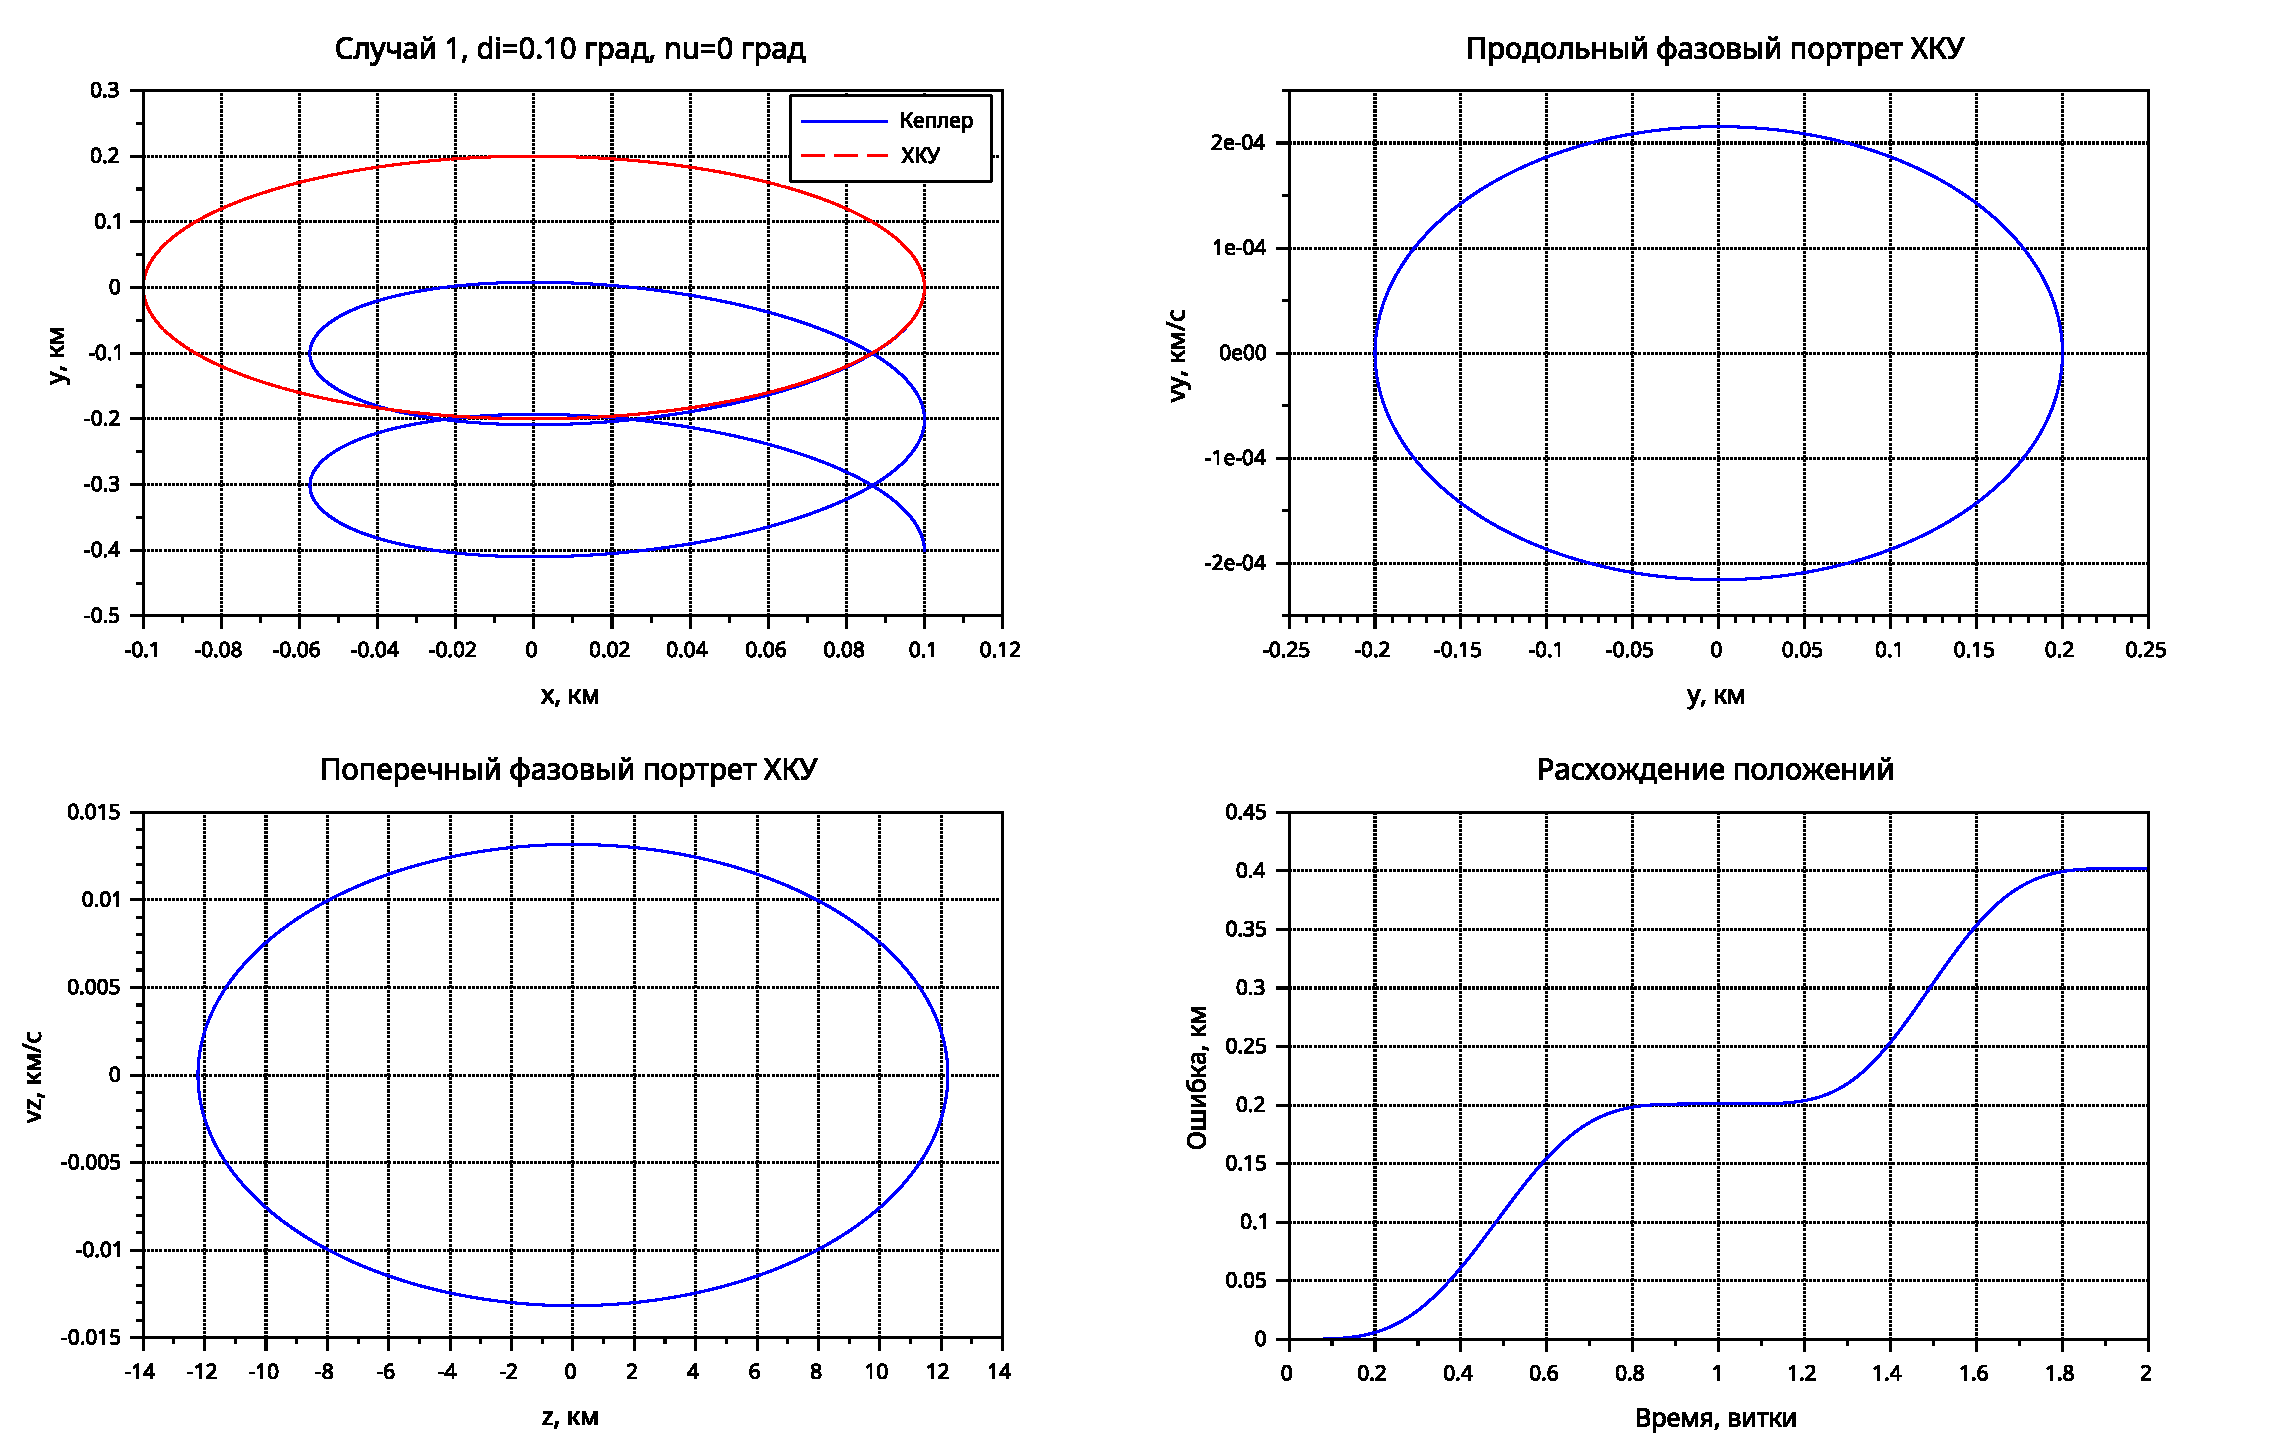
\includegraphics[width=.95\textwidth]{results/case_01_i02_nu000.pdf}\caption{Случай №1: согласованная скорость, $\Delta i=0.1^\circ$, $\nu_0=0^\circ$.}\end{figure}
\begin{figure}[H]\centering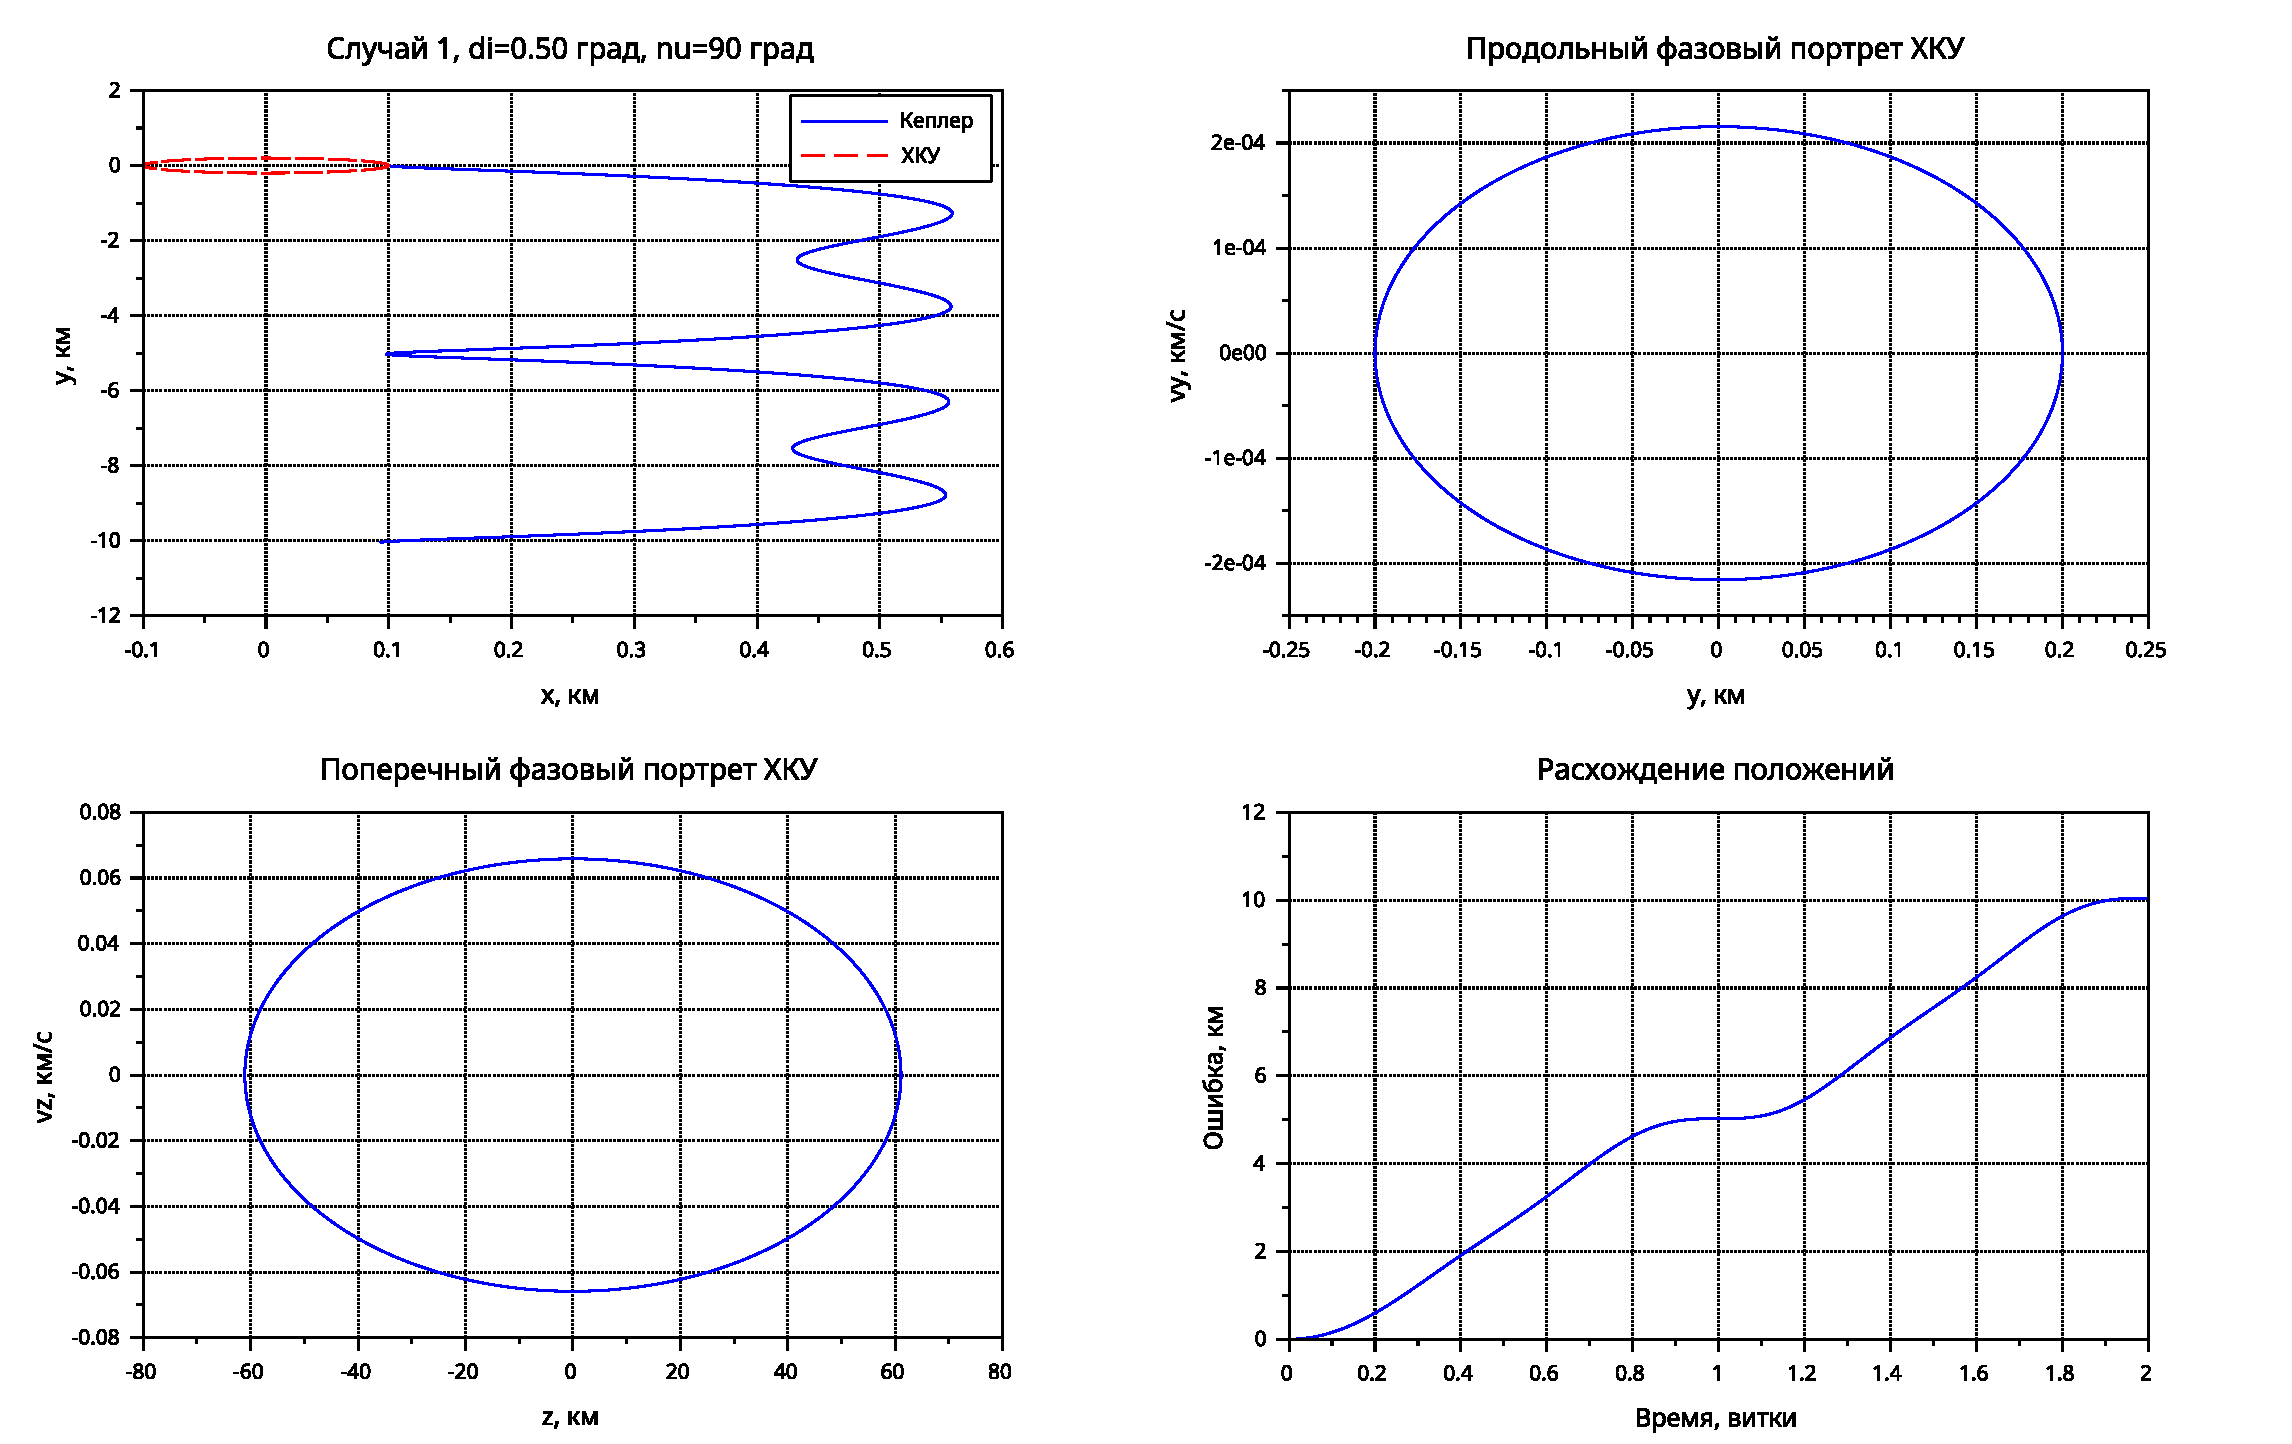
\includegraphics[width=.95\textwidth]{results/case_01_i03_nu090.pdf}\caption{Случай №1: $\Delta i=0.5^\circ$, $\nu_0=90^\circ$.}\end{figure}
\begin{figure}[H]\centering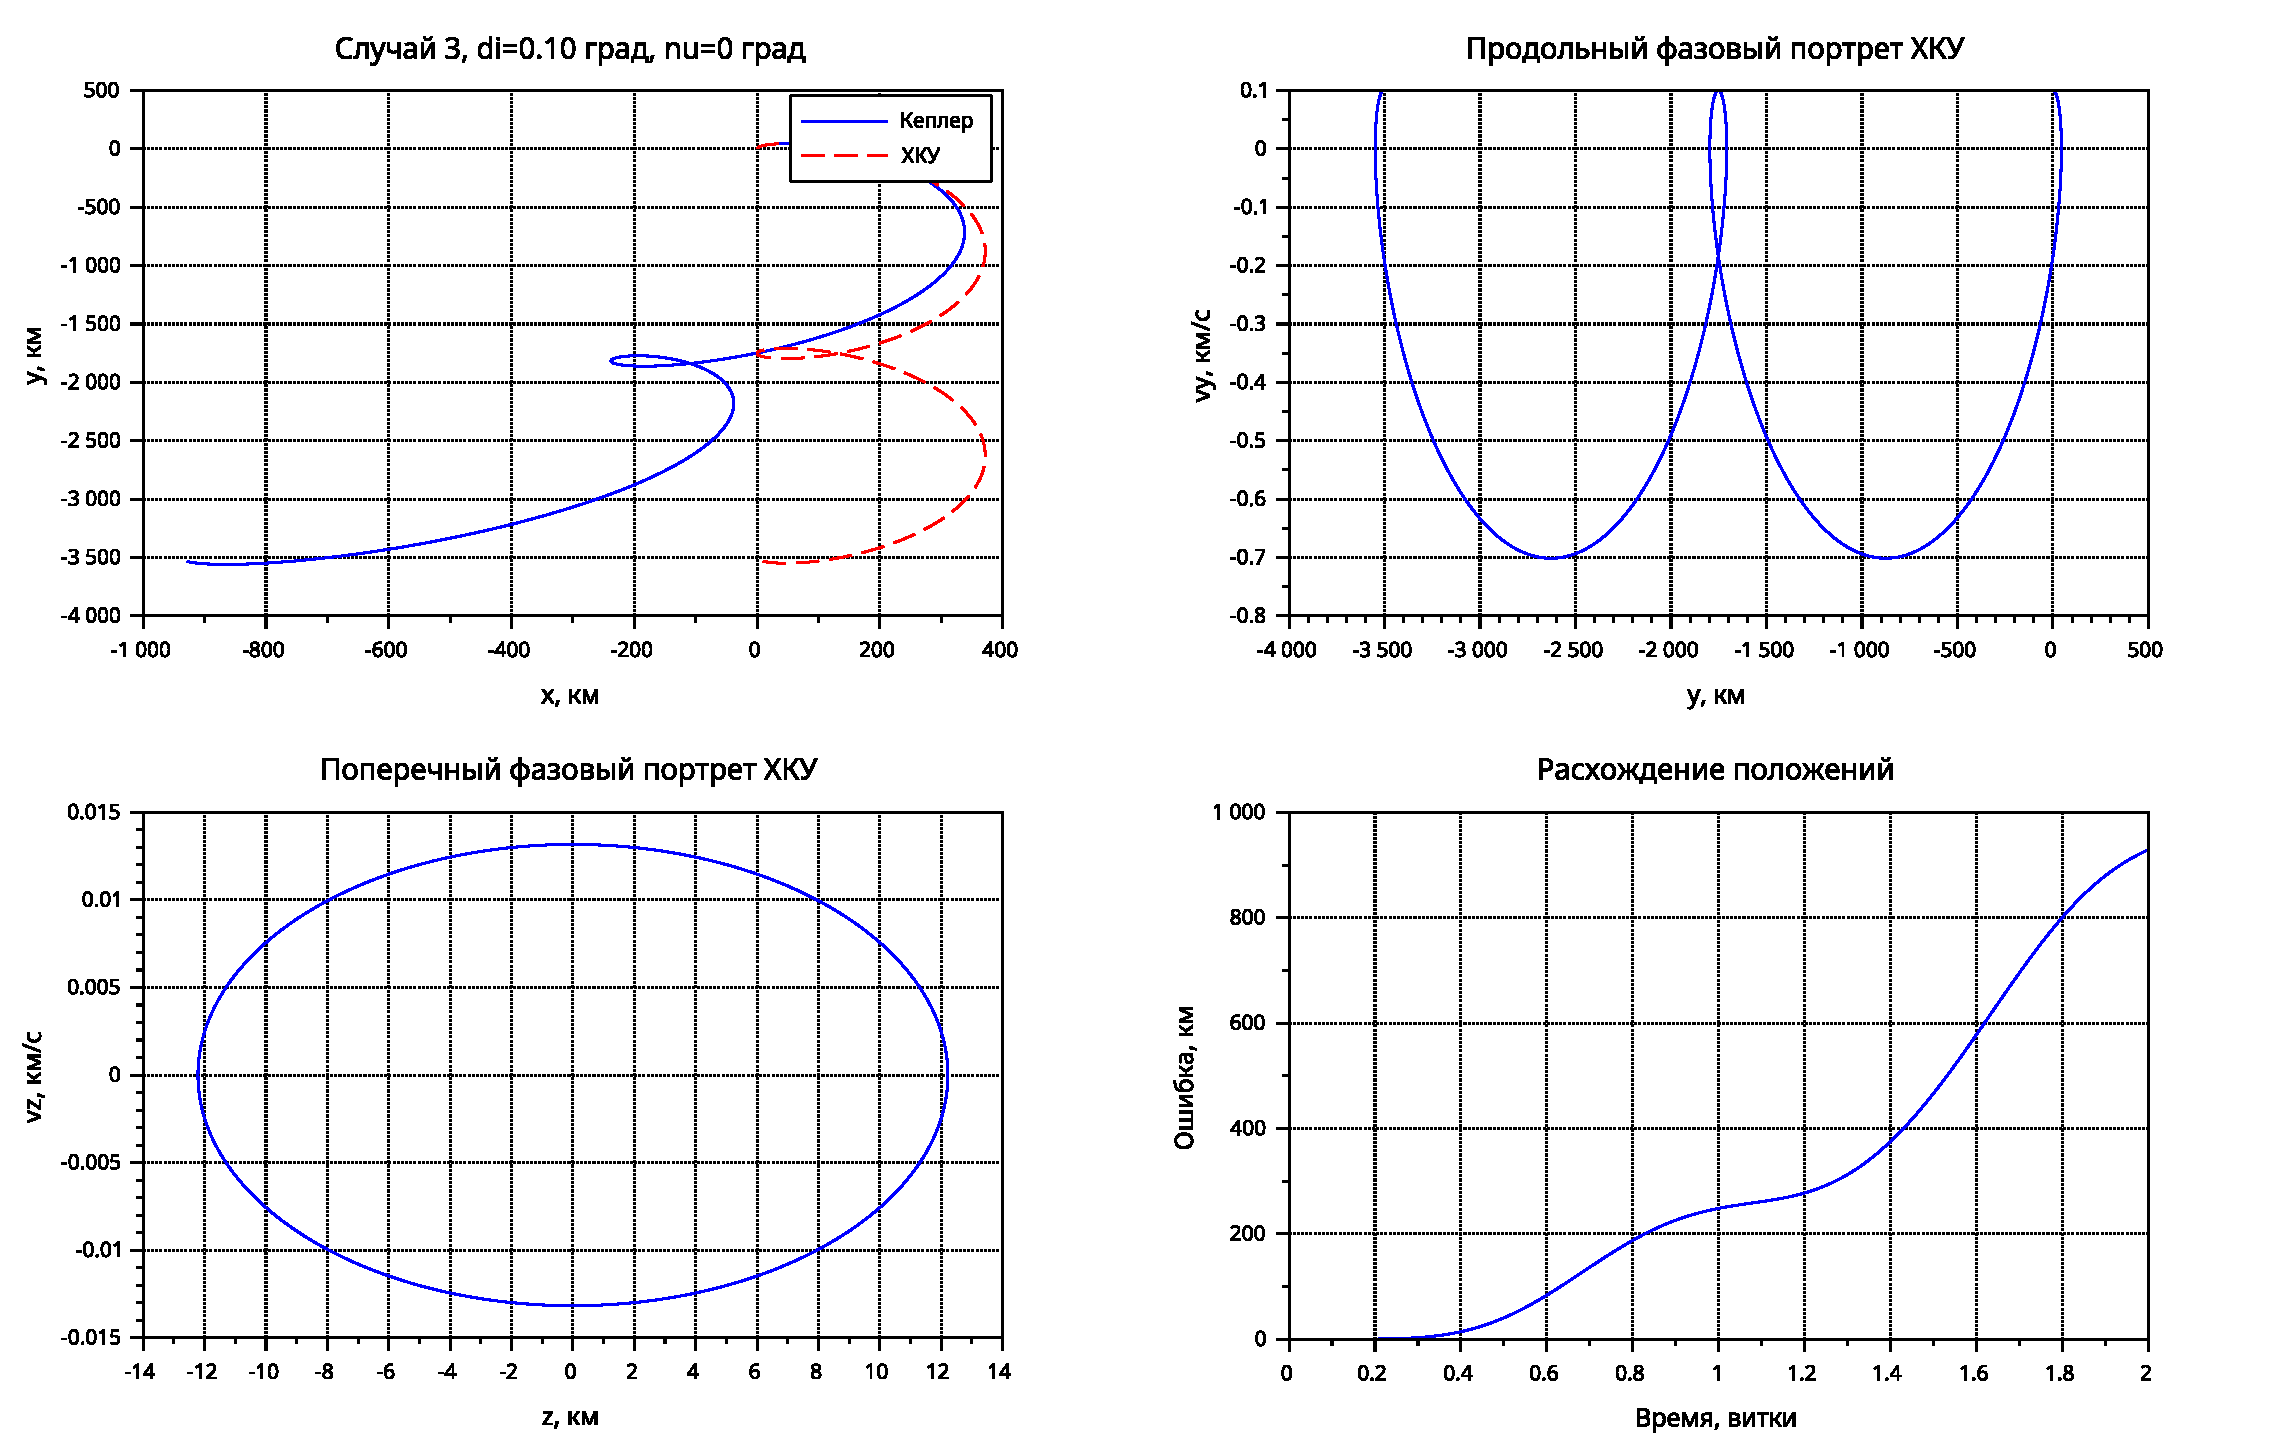
\includegraphics[width=.95\textwidth]{results/case_03_i02_nu000.pdf}\caption{Случай №3: несогласованная продольная скорость, $\Delta i=0.1^\circ$.}\end{figure}
\begin{figure}[H]\centering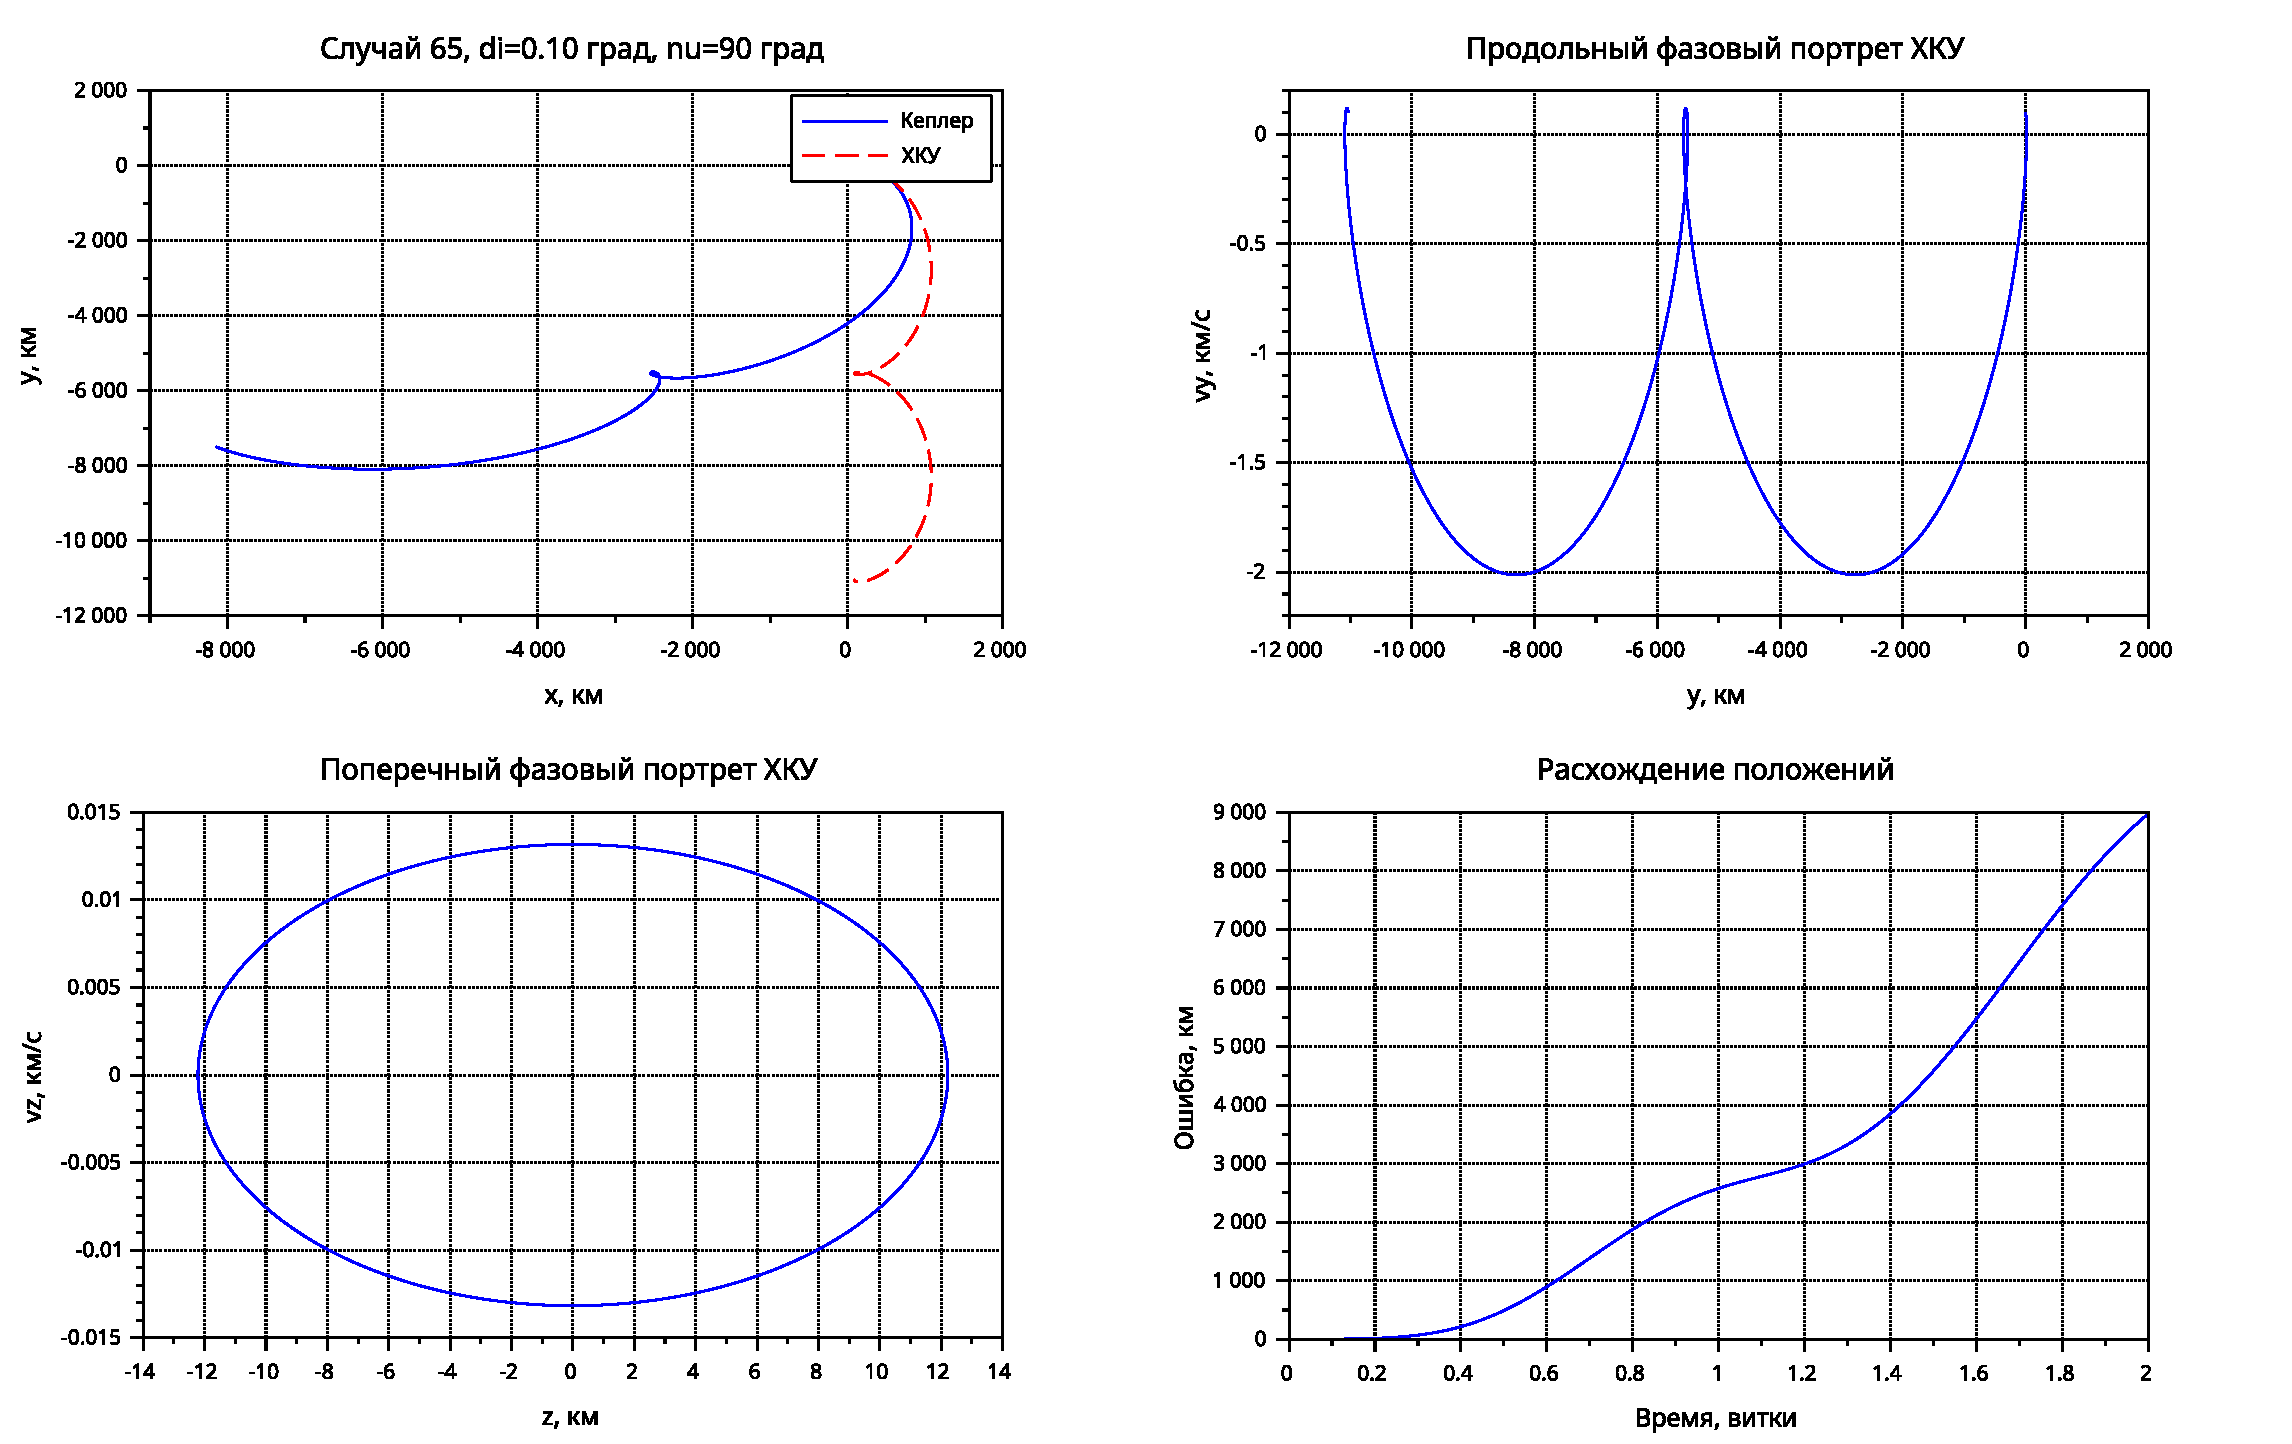
\includegraphics[width=.95\textwidth]{results/case_65_i02_nu090.pdf}\caption{Случай №65: крупное расхождение моделей при $\Delta i=0.1^\circ$.}\end{figure}
\section{Выводы}
\begin{enumerate}
\item Для каждого из трёх базовых случаев из задания 1 рассчитаны 12 комбинаций аномалии и относительного наклонения. Начальные поперечные компоненты получены через инерциальные векторы.
\item В случае №1 условие отсутствия секулярного дрейфа выполняется; однако при увеличении наклонения ошибка относительно двухтельной модели растёт. Замкнутость фазового портрета ХКУ не означает нулевую ошибку линейной модели.
\item Случаи №3 и №65 показывают неприменимость ХКУ для точного прогноза на рассматриваемом интервале: относительное расстояние велико, а ошибка достигает сотен и тысяч километров соответственно.
\item Сравнение выполнено с идеальной двухтельной моделью. Оно не учитывает атмосферу, несферичность Земли и манёвры, поэтому не является оценкой ошибки реального полёта.
\end{enumerate}
\end{document}
